\documentclass{article}
\usepackage{geometry}
\geometry{a4paper}
\geometry{a4paper, left=25.4mm,top=25.4mm, right=25.4mm, bottom=25.4mm}
\usepackage{graphicx}
\usepackage{mathptmx}
\usepackage{enumerate}
\usepackage{pgf,tikz,pgfplots}
\pgfplotsset{compat=1.15}
\usepackage{mathrsfs}
\usetikzlibrary{arrows}
\usepackage[parfill]{parskip}
\usepackage{amsmath, amsthm,amssymb}
\begin{document}
    {\LARGE{MA2108 AY18/19 Semester 2 Exam Suggested Solutions}}
    \vspace{0.2in}
    
    Authors: Chong Jing Quan, Pan Jing Bin \hfill Reviewer: ????
    
    \par\noindent\rule{\textwidth}{0.4pt}
\section*{Question 1}
\begin{enumerate}[(a)]
    \item \begin{enumerate}[(i)]
        \item Note that $\displaystyle(n^28^n+n^34^n)^{\frac{1}{3n}}=n^{\frac{2}{3n}}(8^n+n\times4^n)^{\frac{1}{3n}}.$ Since $\displaystyle\lim_{n\to\infty}n^{\frac{2}{3n}}=1,$ it suffices to compute the limit \newline $\displaystyle\lim_{n\to\infty}(8^n+n\times4^n)^{\frac{1}{3n}}.$
        
        We first show that $2\times8^n>8^n+n\times4^n>8^n$ for all positive integers $n.$ The inequality $8^n+n\times 4^n>8^n$ is obvious. To show that $2\times8^n>8^n+n\times4^n,$ it is equivalent to prove that $8^n>n\times4^n.$ Indeed, the inequality is obvious for $n=1.$ Suppose the inequality holds for $n=k.$ Then $$8^{k+1}=8\times8^k>8(k\times 4^k)>k\times 4^{k+1}$$ and we are done by induction.
        
        Hence, we have $$(2\times8^n)^{\frac{1}{3n}}=2^{\frac{1}{3n}}\times2>(8^n+n\times4^n)^{\frac{1}{3n}}>(8^n)^{\frac{1}{3n}}=2.$$
        Since $\displaystyle\lim_{n\to\infty}2^{\frac{1}{3n}}=1,$ it follows from squeeze theorem that the required limit is 2.
        \item We have
        $$\frac{(n+1)^{2n^2}(n-1)^{2n^2}}{(n^2+1)^{2n^2}}=\frac{(n^2-1)^{2n^2}}{(n^2+1)^{2n^2}}=\left(\frac{n^2-1}{n^2+1}\right)^{2n^2}
        =\left(1-\frac{2}{n^2+1}\right)^{2n^2}
        =\frac{\left(1-\frac{2}{n^2+1}\right)^{2n^2+2}}{\left(1-\frac{2}{n^2+1}\right)^{2}}.$$
        Since $$\lim_{n\to\infty}\left(1-\frac{2}{n^2+1}\right)^{2n^2+2}=\lim_{n\to\infty}\left(\left(1-\frac{2}{n^2+1}\right)^{n^2+1}\right)^2=\left(\lim_{n\to\infty}\left(1-\frac{2}{n^2+1}\right)^{n^2+1}\right)^2=e^{-4}$$ and $$\lim_{n\to\infty}\left(1-\frac{2}{n^2+1}\right)^{2}=1,$$
        it is now easy to see that the required limit is $e^{-4}.$
        \item We have \begin{eqnarray*}\lim_{n\to\infty}\frac{2^n}{\sqrt{9^n+6^{n+2}}-\sqrt{9^n-n}}&=&\lim_{n\to\infty}\frac{2^n\left(\sqrt{9^n+6^{n+2}}+\sqrt{9^n-n}\right)}{9^n+6^{n+2}-(9^n-n)}\\
        &=&\lim_{n\to\infty}\frac{2^n\left(\sqrt{9^n+6^{n+2}}+\sqrt{9^n-n}\right)}{6^{n+2}+n}\\
        &=&\lim_{n\to\infty}\frac{\sqrt{1+\frac{6^{n+2}}{9^n}}+\sqrt{1-\frac{n}{9^n}}}{36+\frac{n}{6^n}}\\
        &=&\frac{\sqrt{1+0}+\sqrt{1-0}}{36+0}\\
        &=&\frac{1}{18}.
        \end{eqnarray*}
    \end{enumerate}
    \item The function is only continuous at $x=3.$ Let $\varepsilon>0$ be given. Take $\delta=\min\left\{1,\dfrac{\varepsilon}{2}\right\}$ so that\\ $0<|x-3|<\delta\implies |f(x)-4|<\varepsilon.$ Indeed, we have $$ |f(x)-4|\leq \sup\left\{\frac{4}{|x-1|}|x-3|,|x-3|\right\}<2|x-2|<2\times\frac{\varepsilon}{2}=\varepsilon.$$ Thus, the function is continuous at $x=3.$
    
    For $x\neq3,$ consider two cases. If $x$ is rational, then $f(x)=\dfrac{8}{x-1}.$ Consider a sequence of irrational numbers $(x_n)^{\infty}_{n=1}$ that converges to $x.$ Then, $f(x_k)=x_k+1$ for each positive integer $k.$ 
    
    Since $x\neq 3,$ the limit $\displaystyle\lim_{k\to\infty}(x_k+1)=x+1$ does not equal to $f(x)=\dfrac{8}{x-1}.$ Thus, the function is not continuous at rational values other than 3. The case for $x$ is irrational can be handled similarly.
\end{enumerate}
\section*{Question 2}
\begin{enumerate}[(a)]
    \item \begin{enumerate}[(i)]
        \item We have $$0<\sqrt{4^n+n^2+1}-2^n=\frac{4^n+n^2+1-4^n}{\sqrt{4^n+n^2+1}+2^n}=\frac{n^2+1}{\sqrt{4^n+n^2+1}+2^n}<\frac{n^2+1}{2^{n+1}}.$$
        Since $\displaystyle\lim_{n\to\infty}\sqrt[n]{\frac{n^2+1}{2^{n+1}}}=\frac{1}{2},$ the series $\displaystyle\sum^{\infty}_{n=1}\frac{n^2+1}{2^{n+1}}$ converges by root test. Hence, the original series converges by comparison test.
        \item Using ratio test, we see that $$L:=\lim_{n\to\infty}\left|\frac{\frac{(2(n+1))!}{(n+1)!(n+1)^{n+1}}}{\frac{(2n)!}{n!n^n}}\right|=\lim_{n\to\infty}2\times\frac{2n+1}{n+1}\times\frac{n^n}{(n+1)^n}.$$
        Since $\displaystyle\lim_{n\to\infty}\frac{2n+1}{n+1}=2$ and $\displaystyle\lim_{n\to\infty}\frac{n^n}{(n+1)^n}=\frac{1}{e},$ we have $L=\dfrac{4}{e}>1.$ Thus, the series diverges.
    \end{enumerate}
    \item We note that the series is an alternating series since $n^2-n-3$ is increasing for $n\geq3$ and $\sin\left(n\pi+\dfrac{\pi}{2}\right)=1$ for even $n$ and $\sin\left(n\pi+\dfrac{\pi}{2}\right)=-1$ for odd $n.$ Hence, the series converges by alternating series test.
    
    However, since for $n>3,$ we have $n^2-n-3<n^2\implies \dfrac{1}{\sqrt{n^2-n-3}}>\dfrac{1}{n},$ the series does not converge absolutely. Hence, the series converge conditionally.
\end{enumerate}

\section*{Question 3}
\begin{enumerate}[(a)]
    \item We first show that $x_n>5$ by induction. The case for $n=1$ is clear. Suppose $x_k>5$ for some positive integer $k.$ We want show that $x_{k+1}>5.$ We have $$x_k>5\implies \frac{3}{x_k}<\frac{3}{5}\implies \frac{3}{x_k}+1<\frac{8}{5}\implies\frac{8}{\frac{3}{x_k}+1}=x_{k+1}>5,$$ which completes the induction step. We now want to show that the sequence converges to $5.$ We have $$|x_{n+1}-5|=\left|\frac{8x_n}{x_n+3}-5\right|=\frac{3}{3+x_n}\left|x_n-5\right|<\frac{3}{8}|x_n-5|.$$ Thus, the sequence contracts and converges to 5.
    \item Define $$f(x)=\begin{cases}
    1&x\leq 0\\
    3x+1&0<x\leq1\\
    -2x+6&1<x\leq2\\
    7x-12&2<x\leq4\\
    -2x+24&4<x\leq8\\
    8&x>8.
    \end{cases}$$
    It is easy to see that $f$ is continuous, $f(x)>0$ for all $x\in\mathbb{R}$ and $f(1)\cdot f(8)=f(2)\cdot f(4).$ However, there is no $c\in[1,2]$ so that $(f(2c))^2=f(c)\cdot f(4c)$ since $$(f(2c))^2=f(c)\cdot f(4c)\implies (7c-12)^2=(-2c+6)(-2c+24)\implies c=0\text{ or }c=\frac{12}{5}.$$
    
    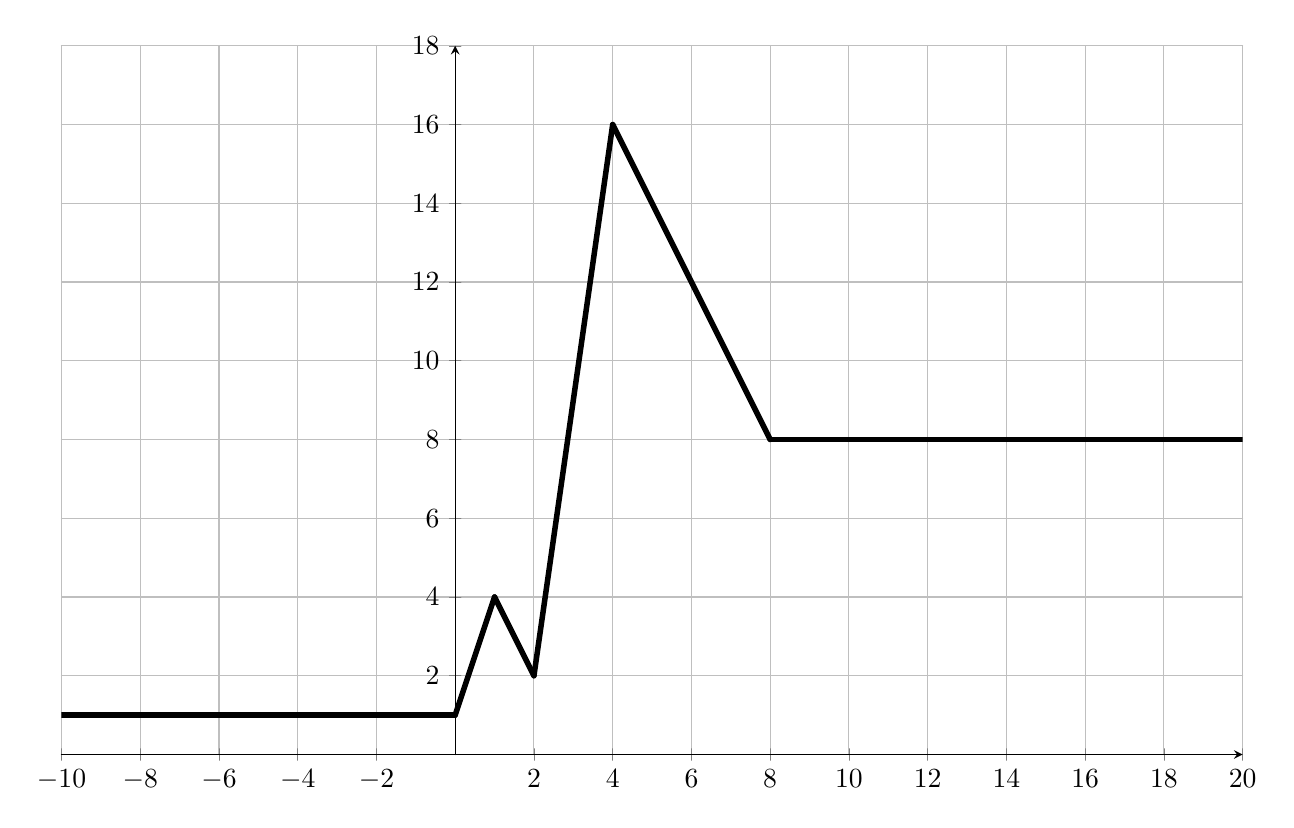
\begin{tikzpicture}[line cap=round,line join=round,>=triangle 45,x=0.5cm,y=0.5cm]
\begin{axis}[
x=0.5cm,y=0.5cm,
axis lines=middle,
ymajorgrids=true,
xmajorgrids=true,
xmin=-10.0,
xmax=20.0,
ymin=0.0,
ymax=18.0,
xtick={-10.0,-8.0,...,20.0},
ytick={0.0,2.0,...,18.0},]
\clip(-10.,0.) rectangle (20.,18.);
\draw [line width=2.pt,domain=-10.0:0.0] plot(\x,{(-7.502978499992442-0.*\x)/-7.502978499992442});
\draw [line width=2.pt,domain=8.0:20.0] plot(\x,{(--61.09066910397955-0.*\x)/7.636333637997444});
\draw [line width=2.pt] (0.,1.)-- (1.,4.);
\draw [line width=2.pt] (1.,4.)-- (2.,2.);
\draw [line width=2.pt] (2.,2.)-- (4.,16.);
\draw [line width=2.pt] (4.,16.)-- (8.,8.);
\end{axis}
\end{tikzpicture}
\begin{center}
    \textit{Graph of $y=f(x)$}
\end{center}
\end{enumerate}
\section*{Question 4}
\begin{enumerate}[(a)]
    \item Suppose $X:=\{x_{g(n)}\}^{\infty}_{n=1}$ and $Y:=\{y_{g(n)}\}^{\infty}_{n=1}$ are two subsequences so that $z=\displaystyle\lim_{n\to\infty}\frac{x_{g(n)}}{y_{g(n)}}.$
    
    Since $X$ and $Y$ are both bounded sequences, by Bolzano-Weierstrass theorem, there exists subsequences $\{x_{f(n)}\}^{\infty}_{n=1}$ and $\{y_{h(n)}\}^{\infty}_{n=1}$ of $X$ and $Y$ respectively so that $\displaystyle\lim_{n\to\infty}x_{f(n)}=x$ and $\displaystyle\lim_{n\to\infty}y_{h(n)}=y.$ In particular, there is no subsequence of $Y$ that converges to 0. Suppose there is one such sequence. Then, for a given $\varepsilon_1>0,$ there exists a positive integer $N$ so that $|y_{k(n)}|<\varepsilon_1$ for all $n\geq N.$ Hence, $\left|\dfrac{x_{k(n)}}{y_{k(n)}}\right|>\dfrac{1}{\varepsilon_1},$ which contradicts the fact that $\left|\dfrac{x_{k(n)}}{y_{k(n)}}\right|$ is bounded. Now, it is easy to check that $\dfrac{x}{y}=z.$
    %\item Firstly, note that $f(x) = f(\frac{x+2}{3})$ for all $x$ and denote $g(a) = \frac{a+2}{3}$. Let $f(1) = a$. Suppose there exists $y$ so that $y \neq 1$ and $f(y) \neq a$. WLOG $y>1$. By continuity, there exists $\delta$ such that $|x-1| < \delta \implies |f(x)-f(1)| < \frac{f(a)-f(1)}{2}$. Let $|a-1| = A$. Then, $|g(a)-1| = \frac{A}{3}$ and more generally, $|g^n(a)-1| = \frac{A}{3^n}$, which obviously limits to zero as $n$ approaches infinity. However, by the condition of the problem, $|f(g^n(a))-f(1)|$ is a nonzero constant for all $n$, contradicting the continuity at 1.% Solution added by Jessen
    \item The statement is true. Let $\varepsilon>0$ be given. Then, there exists $\delta_1$ so that $|x-y|<\delta_1\implies |g(x)-g(y)|<\varepsilon.$ On the other hand, since $f$ is continuous on $[0,1],$ $f$ is uniformly continuous on $[0,1].$ Then, there exists $\delta_2$ so that $|x-y|<\delta_2\implies |f(x)-f(y)|<\delta_1.$ Consequently, $|x-y|<\delta_2\implies |h(x)-h(y)|=|g\circ f(x)-g\circ f(y)|<\varepsilon.$
\end{enumerate}
\section*{Question 5}
\begin{enumerate}[(a)]
    \item \begin{enumerate}[(i)]
        \item The limit is $12\cos 5.$ Clearly, $$\lim_{x\to 5^-}\cos x=\lim_{x\to 5^+}\cos x=\lim_{x\to 5}\cos x=\cos 5.$$
        Now, we examine the limit $L:=\displaystyle\lim_{x\to 5}\left(\lfloor2x\rfloor+\left\lfloor\dfrac{75}{x^2}\right\rfloor\right).$ Observe that $$\lim_{x\to 5^-}\left(\lfloor2x\rfloor+\left\lfloor\dfrac{75}{x^2}\right\rfloor\right)=\lim_{x\to 5^-}\lfloor2x\rfloor+\lim_{x\to 5^-}\left\lfloor\dfrac{75}{x^2}\right\rfloor=9+3=12$$
        and $$\lim_{x\to 5^+}\left(\lfloor2x\rfloor+\left\lfloor\dfrac{75}{x^2}\right\rfloor\right)=\lim_{x\to 5^+}\lfloor2x\rfloor+\lim_{x\to 5^+}\left\lfloor\dfrac{75}{x^2}\right\rfloor=10+2=12.$$
        Hence, $L=12.$ Thus, the final limit is $12\cos5.$
        \item We show that the limit $\displaystyle\lim_{x\to3}\sin\left(\frac{x}{3-x}\right)$ does not exist. Let $L$ be the limit and let $\varepsilon=1$. Suppose $L\geq 0.$ Then, for each positive integer $n,$ we see that if $x=\dfrac{\frac{9\pi}{2}+6n\pi}{1+\frac{3\pi}{2}+2n\pi},$ then $\sin\left(\dfrac{x}{3-x}\right)=-1.$ In fact, for any $\delta>0,$ there exists a positive integer $N$ so that $|x-3|=\dfrac{3}{1+\frac{3\pi}{2}+2n\pi}<\delta$ for all $n\geq N.$ Thus, we get $\displaystyle\left|\sin\left(\frac{x}{3-x}\right)-a\right|\geq1=\varepsilon.$  The proof is similar for $L<0.$
        
        Suppose the limit $\displaystyle\lim_{x\to3}(x+1)\sin\left(\frac{x}{3-x}\right)$ exists. Then, we see that $\displaystyle\lim_{x\to3}(x+1)\sin\left(\frac{x}{3-x}\right)\cdot\frac{1}{x+1}=\displaystyle\lim_{x\to3}\sin\left(\frac{x}{3-x}\right)$ also exists since $\displaystyle\lim_{x\to3}\frac{1}{x+1}$ exists. This is a contradiction and we are done.
    \end{enumerate}
    \item We prove that $\displaystyle\lim_{x\to\infty}f(x)=\sup\{f(x):x\in[1,\infty)\}.$
\end{enumerate}
\section*{Question 6}
\begin{enumerate}[(a)]
        \item Let $\varepsilon>0$ be given. Then choose $\delta=\min\left\{\dfrac{1}{4},2\varepsilon\right\}$ so that $0<|x-2|<\delta\implies\left|\dfrac{x^2-6}{2x-5}-2\right|<\varepsilon.$ We have
        $$\left|\dfrac{x^2-6}{2x-5}-2\right|=\left|\frac{x^2-4x+4}{2x-5}\right|=
        \left|\frac{(x-2)^2}{2x-5}\right|=|x-2|\left|\frac{x-2}{2x-5}\right|<\frac{1}{2}|x-2|<\frac{1}{2}\times2\varepsilon=\varepsilon.$$
        The result follows.
        \item WHAT THIS?
\end{enumerate}
\end{document}